\chapter{DATA COLLECTION}\label{chap-data}
\thispagestyle{empty}

This chapter describes the data collected for the design and implementation of the Cold Plasma Generator. It covers input parameters, specifications of components, experimental observations, and sources of reference data. The reliability and adequacy of the data used for simulation, design calculations, and prototype development are also discussed.

\section{Electrical Specifications and Parameters}

The key electrical parameters required for the design of the high-voltage pulsed power supply and plasma jet are summarized in Table~\ref{tab-electrical}. These were obtained from datasheets, manufacturer manuals, and previous literature \cite{Diaz2022}, \cite{Spassov1997}.

\begin{table}[h!]\centering
\caption{Electrical Specifications for Cold Plasma Generator}
\label{tab-electrical}
\begin{tabular}{|l|l|}
\hline
Parameter & Value \\ \hline
Input Voltage, $V_{in}$ & 230~V AC \\ \hline
Output Voltage, $V_{HV}$ & 30~kV DC \\ \hline
Switching Frequency, $f_{sw}$ & 100~kHz \\ \hline
Output Power & 150--250~W \\ \hline
Microcontroller & LAUNCHXL-F28379D \\ \hline
MOSFET & IRFP460 \\ \hline
Gate Driver & UCC21330 \\ \hline
Working Gas & Argon (Ar) \\ \hline
\end{tabular}
\end{table}

\section{Mechanical and Gas Flow Data}

For plasma jet formation, mechanical parameters such as nozzle diameter, distance from target, and argon flow rate were collected from literature \cite{Cheng2006} and vendor specifications. A typical argon flow rate of 1–3~slm (standard liters per minute) was used to sustain a stable plasma jet.

\section{Experimental Observations}

Prototype testing provided the following observed data:
\begin{itemize}
    \item H-bridge switching waveform measured at the MOSFET drain using an oscilloscope.
    \item High-voltage output waveform after the Cockcroft--Walton multiplier.
    \item Plasma jet length, visibility, and stability at different voltages and argon flow rates.
\end{itemize}

\section{Figures and Tables}

Fig.~\ref{fig-hbridge} shows the schematic of the IRFP460 H-bridge circuit used in the project.  

\begin{figure}[h!]
\centering
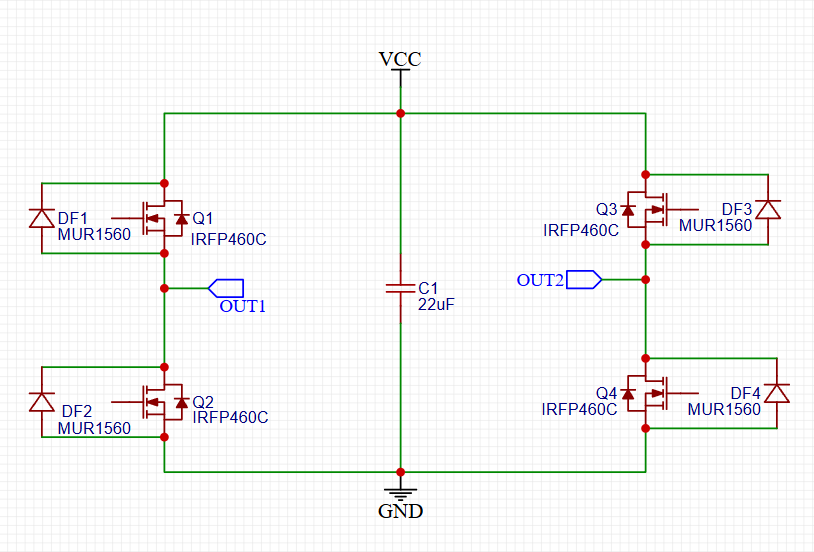
\includegraphics[width=1\linewidth]{./picture-files/hbridge-schematic1.png}
\caption[Schematic of IRFP460 H-Bridge]{H-Bridge schematic used to drive high-voltage transformer}
\label{fig-hbridge}
\end{figure}
\clearpage


Tables~\ref{tab-electrical} and \ref{tab-experimental} summarize the collected specifications and experimental observations.

\begin{table}[h!]\centering
\caption{Experimental Observations}
\label{tab-experimental}
\begin{tabular}{|l|l|}
\hline
Observation & Value \\ \hline
Peak HV Output & 30.2~kV DC \\ \hline
Plasma Jet Length & 5--7~cm \\ \hline
Switching Waveform & 100~kHz square wave \\ \hline
Voltage Control Range & 10--30~kV \\ \hline
\end{tabular}
\end{table}

